\documentclass{article}
\usepackage[left=2cm, right=2cm]{geometry}
\usepackage{multicol}
\usepackage{graphicx}
\usepackage{subcaption}
\usepackage{listings}

\setlength{\columnsep}{1.5cm}

\lstdefinestyle{mystyle}{
    basicstyle=\tiny,
    breakatwhitespace=false,
    breaklines=true,            
    tabsize=1,
    frame=single
}
 
\lstset{style=mystyle}

\title{
    \textbf{Programação 3D} \\
    Relatório Técnico da Primeira Entrega
}
\author{Afonso Mercier \and Pedro Quintas \and Pedro Caldeira}
\date{}

\begin{document}
    \maketitle

    \begin{multicols}{2}
    \section{Funcionamento do Programa}

    O trabalho desenvolvido consiste numa aplicação de ray tracing na linguagem
    C++. O programa pode ser configurado para ler um ficheiro NFF e produz uma
    imagem fotorrealista com base na cena descrita no ficheiro.

    O desenvolvimento focou-se nos seguintes aspetos:

    \begin{itemize}
        \item Leitura de ficheiros NFF.
        \item Cálculo dos Raios Primários
        \item Cálculo da componente local da cor.
        \item Suporte para multiplas fontes luminosas.
        \item Sombras de contorno rígido.
        \item Reflecção de raios.
        \item Refracção de raios.
        \item Intersecções de raios com algumas primitivas.
        \begin{itemize}
            \item Esferas
            \item Planos Infinitos
            \item Triângulos
            \item AABBs
        \end{itemize}
    \end{itemize}

    \section{Leitura de Ficheiros NFF}
    
    Ipsum Lorem

    \section{Raios Primários}

    Ipsum Lorem

    \section{Componente Local da Cor}

    Caso um raio não intersecte nenhum objecto da cena, a sua cor corresponde
    à cor de fundo. No entanto, assim que é detectada uma intersecção, a
    primeira coisa a fazer é calcular a componente local da cor. Isto é a cor
    que resulta diretamente da influência das luzes da cena sobre o material
    do objecto.

    Para isto utilizamos o modelo de iluminação de Blinn-Phong. Este consiste no
    cálculo das componentes difusa e especular da cor. A componente difusa depende
    da direcção da luz e da normal no ponto e é dada por
    $ Cor_{difusa} = k_d (\vec{n} \cdot \vec{l}) \cdot Cor_{material} $.

\begin{lstlisting}[language=C++]
float diffuse_c = clamp(col.object->_matProps->diffuseComp * internalProduct(col.normal, lightDirection), 0, 1);
Color diffuse = colorTimesConstant(col.object->_matProps->color, diffuse_c);
color = addColors(color, diffuse);
\end{lstlisting}

    A componente especular depende da normal e do vector \textit{halfway}, que fica a meio
    entre a direcção do raio e a direcção da fonte luminosa, e é dada por
    $ Cor_{especular} = k_e (\vec{n} \cdot \vec{h})^{shine} \cdot Cor_{luz} $.

\begin{lstlisting}[language=C++]
Vector3 halfway = normalize(addVector(lightDirection, vector3MultScalar(ray.versor, -1)));

if (col.object->_matProps->specularComp > 0) {
    float specular_c = col.object->_matProps->specularComp * pow(internalProduct(col.normal, halfway), col.object->_matProps->shine);
    Color specular = colorTimesConstant(light->color, specular_c);
    color = addColors(color, specular);
}
\end{lstlisting}

    \section{Fontes Luminosas}

    Ipsum Lorem

    \section{Sombras}

    Para calcular as sombras de contorno rígido, basta garantir que cada uma das fontes
    luminosas é efectivamente capaz de iluminar o ponto no qual estamos a calcular a
    iluminação. Para tal lançamos um raio auxiliar em direcção à fonte luminosa, um
    \textit{shadow feeler}. Caso este raio intersecte algum objecto da cena antes de
    alcançar a fonte luminosa, esta fonte não tem impacto na cor final do ponto.

\begin{lstlisting}[language=C++]
Vector3 lightDirection = normalize(subVector(light->pos, col.point));
if (internalProduct(lightDirection, col.normal) <= 0) {
    // The Light is behind our object.
    continue;
}

Ray shadow_feeler;
shadow_feeler.versor = lightDirection;
shadow_feeler.origin = addVector(col.point, vector3MultScalar(lightDirection, EPSILON));
Collision shadow = scene->castRay(shadow_feeler);

// If the shadow feeler did not collide or if the collision was further away than the light source.
//Bling Phong model
if (shadow.object == nullptr || vector3Length(subVector(shadow_feeler.origin, shadow.point)) > vector3Length(subVector(light->pos, col.point))) {
    // Calculate the Blinn-Phong.
}
\end{lstlisting}

    É também de notar que caso o próprio objecto esteja a tapar a fonte luminosa, esta não
    tem impacto na cor final do objecto.

    \section{Reflecção}
    
    Quando um raio intersecta um objecto, caso a componente especular do material
    seja superior a zero, é necessário calcular a cor relativa à reflecção da
    cena no objecto. Este calculo é feito através de uma chamada recursiva à função
    \verb|rayTracing| utilizando um novo raio. O novo raio é calculado de modo
    a fazer um ângulo com a normal na colisão igual ao ângulo entre o raio incidente
    e a normal na colisão.

    A cor resultante desta reflecção é atenuada de acordo com a componente especular
    do material do objeto.

\begin{lstlisting}[language=C++]
if (col.object->_matProps->specularComp > 0 && depth < DEPTH_TRACE_LIMIT) {
    Ray reflector;
    reflector.versor = normalize(subVector(ray.versor, vector3MultScalar(col.normal, 2 * internalProduct(ray.versor, col.normal))));
    reflector.origin = addVector(col.point, vector3MultScalar(reflector.versor, EPSILON));

    Color reflected = colorTimesConstant(rayTracing(reflector, depth + 1, RefrIndex), col.object->_matProps->specularComp);
    color = addColors(color, reflected);
}
\end{lstlisting}

    O raio criado é ligeiramente deslocado, de modo a evitar intersecções com o objecto reflector. Dada a natureza recursiva do algoritmo de \textit{Ray Tracing} é necessário
    limitar a profundidade que o algoritmo pode alcançar.

    \section{Refracção}

    Quando um raio intersecta um objecto translúcido a sua direcção é alterada
    de acordo com a lei de Snell. Visto que um raio tem uma direcção única, é criado
    um novo raio e a cor resultante deste raio é atenuada de acordo com
    a transmitância do objecto. A direcção do novo raio é resultante da aplicação
    da lei de Snell, $\eta_1/\eta_2 = sin(\theta_1)/sin(\theta_2)$.

\begin{lstlisting}[language=C++]
if (col.object->_matProps->t > 0 && depth < DEPTH_TRACE_LIMIT) {
    Ray refractor;

    float origin_ior = RefrIndex;
    float dest_ior = col.inside ? 1.0f : col.object->_matProps->idxOfRefraction;
    Vector3 v = vector3MultScalar(ray.versor, -1);
    float ior = origin_ior / dest_ior;
    Vector3 vt = subVector(vector3MultScalar(col.normal, internalProduct(v, col.normal)), v);
    float sin_theta_t = ior * vector3Length(vt);
    float cos_theta_t = sqrt(1 - sin_theta_t * sin_theta_t);
    Vector3 t = normalize(vt);

    refractor.versor = normalize(addVector(vector3MultScalar(t, sin_theta_t), vector3MultScalar(col.normal, -cos_theta_t)));
    refractor.origin = addVector(col.point, vector3MultScalar(refractor.versor, EPSILON));

    Color refracted = colorTimesConstant(rayTracing(refractor, depth + 1, dest_ior), col.object->_matProps->t);
    color = addColors(color, refracted);
}
\end{lstlisting}

    Para aplicar a lei de Snell é necessário primeiro descobrir os índices de
    refracção do meio em que o raio está a viajar e do novo meio em que o raio
    vai entrar. Convenientemente, a função \verb|rayTrace| tem como argumento
    o índice de refracção do material em que o raio se está a propagar. O
    índice de refracção do novo material pode ser ou o índice de refracção
    do objecto que o raio intersectou, caso a colisão tenha acontecido fora
    do objecto, ou o índice de refracção do ar, caso a colisão tenha acontecido
    dentro do objecto.

    Tal como com a reflecção, é necessário deslocar ligeiramente o raio refractado
    de modo a evitar intersecções com o próprio objecto.

    \section{Intersecções}

    Ipsum Lorem

    \subsection{Esferas}

    Ipsum Lorem

    \subsection{Planos Infinitos}

    Ipsum Lorem

    \subsection{Triângulos}

    Ipsum Lorem

    \subsection{AABBs}

    Ipsum Lorem

    \end{multicols}

    \newpage
    \section{Imagens}

    \begin{figure}[h!]
        \centering
        \begin{subfigure}{.2\linewidth}
            \centering
            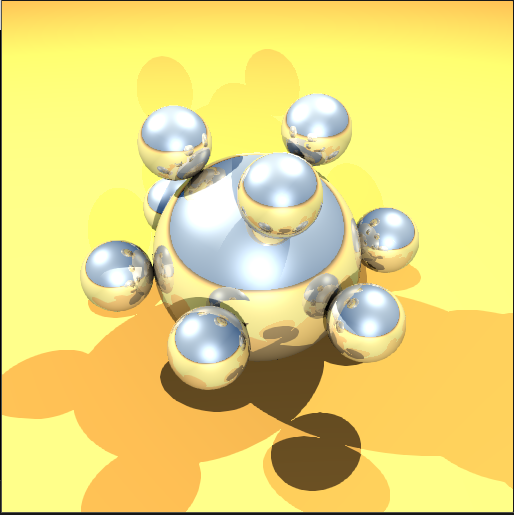
\includegraphics[width=\linewidth]{balls_low.png}
            \caption{balls\_low.nff}
            \label{fig:balls_low}
        \end{subfigure}
        \begin{subfigure}{.2\textwidth}
            \centering
            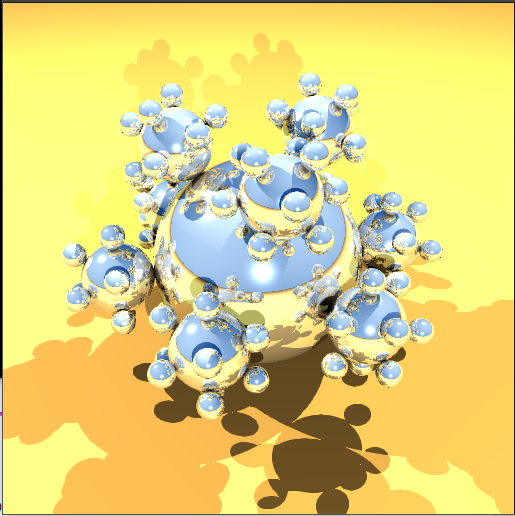
\includegraphics[width=\linewidth]{balls_medium.png}
            \caption{balls\_medium.nff}
            \label{fig:balls_medium}
        \end{subfigure}
        \begin{subfigure}{.2\linewidth}
            \centering
            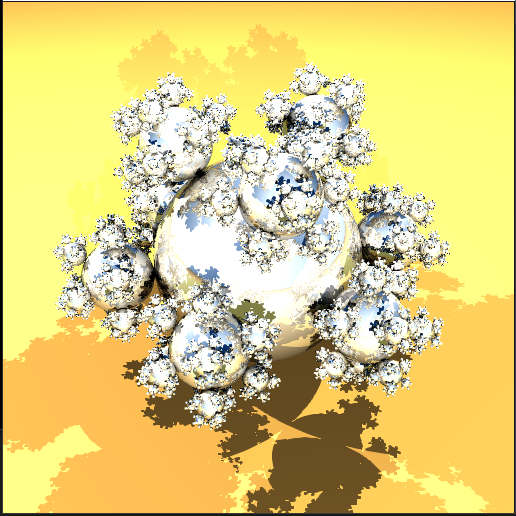
\includegraphics[width=\linewidth]{balls_high.png}
            \caption{balls\_high.nff}
            \label{fig:balls_high}
        \end{subfigure}

        \caption{Reflecções}
        \label{fig:balls}
    \end{figure}

    \begin{figure}[h!]
        \centering
        \begin{subfigure}[b]{.2\linewidth}
            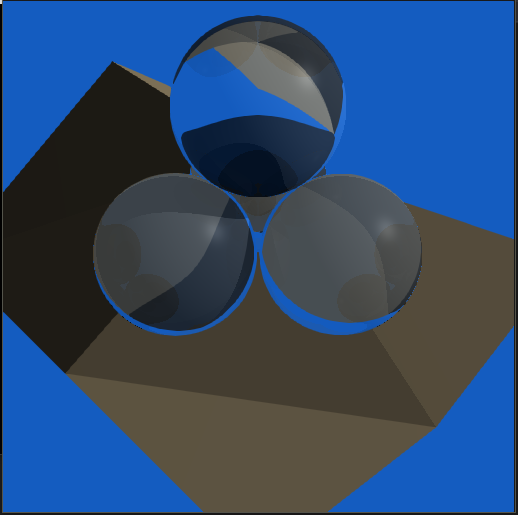
\includegraphics[width=\linewidth]{mount_low.png}
            \caption{mount\_low.nff}
            \label{fig:mount_low}
        \end{subfigure}
        \begin{subfigure}[b]{.2\linewidth}
            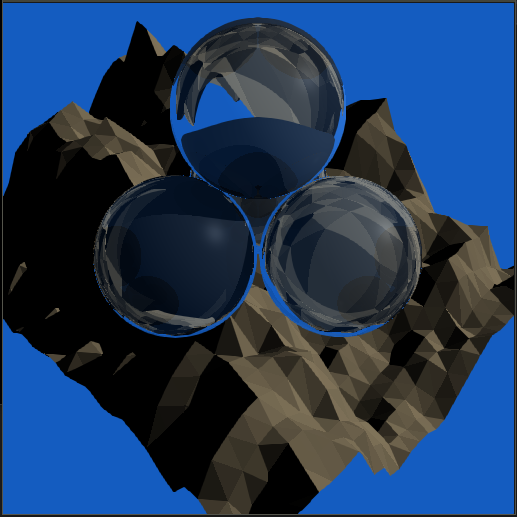
\includegraphics[width=\linewidth]{mount_high.png}
            \caption{mount\_high.nff}
            \label{fig:mount_high}
        \end{subfigure}
        \begin{subfigure}[b]{.2\linewidth}
            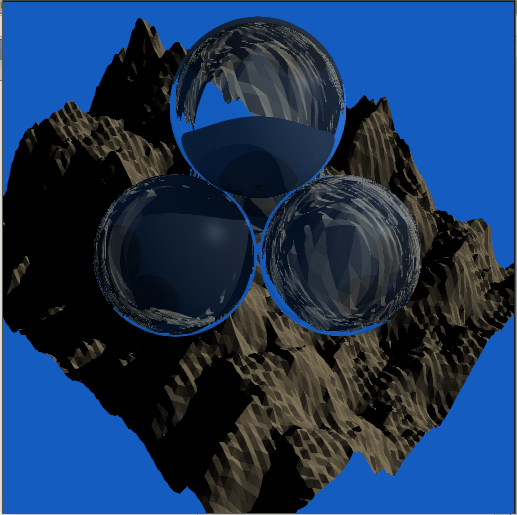
\includegraphics[width=\linewidth]{mount_very_high.png}
            \caption{mount\_very\_high.nff}
            \label{fig:mount_very_high}
        \end{subfigure}

        \caption{Refracções}
        \label{fig:balls}
    \end{figure}

    \begin{figure}[h!]
        \centering
        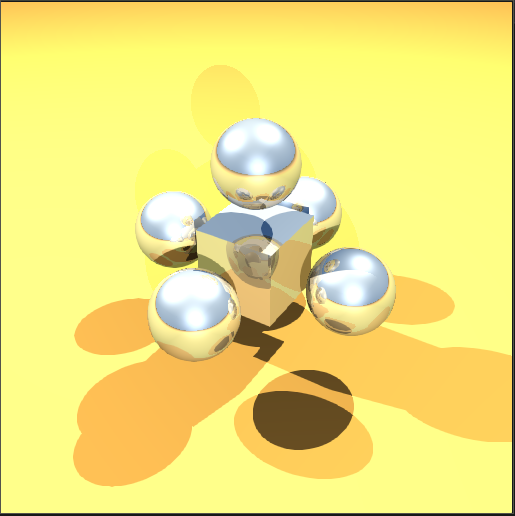
\includegraphics[width=.2\linewidth]{aabb.png}
        \caption{aabb.nff}
        \label{fig:aabb}
    \end{figure}

\end{document}